\documentclass[oribibl]{llncs}
\usepackage[utf8]{inputenc}
\usepackage{llncsdoc}
\usepackage{url}
\usepackage{amsmath}
\usepackage{amssymb}
\usepackage{graphicx}
\usepackage{wrapfig}
\usepackage[cache=false,outputdir=.texpadtmp]{minted}
%
\author{Lennard Wolf \\
        lennard.wolf@student.hpi.de}
\institute{ Hasso Plattner Institute \\
            Prof.-Dr.-Helmert-Straße 2-3 \\
            14482 Potsdam \\
            Germany}
\title{Describing Dynamic Organizational Structures \\
 through the Common Lisp Object System}
\date{\today}
%
\begin{document}
\markboth{Describing Dynamic Organizational Structures \\
 through the Common Lisp Object System}{Describing Dynamic Organizational Structures \\
 through the Common Lisp Object System}
\thispagestyle{empty}
\vfill

%
\maketitle
%
\begin{abstract}
Describing Dynamic Organizational Structures through the Common Lisp Object System Describing Dynamic Organizational Structures through the Common Lisp Object System Describing Dynamic Organizational Structures through the Common Lisp Object System Describing Dynamic Organizational Structures through the Common Lisp Object System Describing Dynamic Organizational Structures through the Common Lisp Object System Describing Dynamic Organizational Structures through the Common Lisp Object System Describing Dynamic Organizational Structures through the Common Lisp Object System
\end{abstract}
%


\section{Introduction}


\begin{itemize}
\item Topic / Domain
\item Problem
\item Contribution
\item Outline (The following is a summary of each Section. In Section...)
\end{itemize}


\section{Problem}
\label{sec:problem}

To achieve their goals, organizational structures require planning as well as control over processes and the network of shareholders. \cite[42f.]{Schmidt2000} To gain the necessary overview, it is often useful to have a list of all members and their roles. 

Since organizations are often dynamic, such a list should also be easily \emph{maintainable}, meaning that participants can be both added or removed as well as change their role. It should also be \emph{extendable} meaning that new roles can easily added and combined with already existing ones. Furthermore, computer programs used within the organization might have to interact with the list, so \emph{accessibility} is another key requirement. These \emph{evolution qualities} \cite{young2001effective} would thus be the key requirements for  any list describing the participants within an organizational structure.


\section{Background}
\label{sec:background}
A solution to the problem introduced in Section \ref{sec:problem} which would meet all the given requirements would be the employment of the \emph{Common Lisp Object System} (CLOS), an extension to Common Lisp\footnote{\url{https://common-lisp.net}, accessed: 2016-07-12} providing "full" object-orientation. \cite{demichiel1987common} However, to understand its utilization in such a problem domain as well as the reasoning behind that, some background information will be needed first.

In this Section we will hence start out by introducing the general ideas behind object-orientated programming languages, as well as the language Lisp, which is followed by a description of the three main concepts that make CLOS unique. An overview of the history of CLOS will be provided thereafter, so as to better understand its origins and historical context.

\subsection{Object-Orientated Languages}
\label{sec:oo}

A definition of \emph{object-orientated} programming languages requires a preceding explanation of the terms \emph{object}, \emph{class}, and \emph{inheritance}. \emph{Objects} have a set of \emph{attributes} that define its \emph{state}, as well as a number of \emph{messages}\footnote{In CLOS, these are referred to as callable \texttt{methods}.} that it can receive to evoke certain behavior. By sending such messages, objects can interact with one another. \emph{Classes} are templates for objects, so that objects of the same class can have uniform interfaces and behavior. An object is hence an \emph{instance} of a class. \emph{Inheritance} opens up the possibility to create class hierarchies, so that classes can be specializations of others and \emph{inherit} certain behavior while adding something unique. The inheriting class is called the \emph{subclass}, the other the \emph{superclass}.

An \emph{object-orientated} programming language is one that has these three concepts "integrated". They give programmers the ability to model human language based conceptualizations of the real world, since these are also just separations of phenomena into groups with common traits.

\subsection{Lisp}
\label{sec:lisp}

Stemming from the term \textbf{Lis}t \textbf{P}rocessor, Lisp is a programming language in which \emph{everything is a list}. This means that there is \emph{no discernment between data and code}. Hence an expression such as \mintinline{lisp}{(plus 3 4)} is without context nothing more than a "meaningless" listing of the "meaningless" expressions \mintinline{lisp}{plus}, \mintinline{lisp}{3}, and \mintinline{lisp}{4}. An expression like that only gets its meaning from an \emph{evaluation} by the interpreter which considers it in a certain context. In such a context the expression \mintinline{lisp}{plus} could be a function to add the arguments it is given, but that is entirely arbitrary. 

Common Lisp is a standardized version of Lisp which provides certain data types and operations. But this type system can be extended through the use of \emph{macros}, which let developers give meaning to expressions. This feature of Lisp greatly facilitates the creation \emph{Domain Specific Languages}. \cite{fowler2011domain-specific} They also form the basis of CLOS which in its entirety consists of 8 macros and 33 functions.


\textbf{explain Macros in detail?}

%reasoning why before concepts: the loops and s.o. are introduced which are needed later on

\subsection{History of CLOS}
\label{sec:history}

In the late 1960s, the new concept of object-orientation started to become a topic of interest for researchers in computer science. In 1986, four major attempts, namely New Flavors\footnote{Information on its predecessor Flavors can be found in \cite{Moon:1986:OPF:28697.28698}.}, CommonLoops\footnote{Information on CommonLoops can be found in \cite{Bobrow:1986:CML:28697.28700}.}, Object Lisp (LMI), and Common Objects, were made to bring that concept to the popular and easily extendable programming language Lisp. \cite{steele1993evolution} To create a standardized object system, researchers from Symbolics, Inc. and Xerox PARC met to combine their respective object systems, New Flavors and CommonLoops. \cite{demichiel1987common} The Common Lisp Object System was the result, which had been two years in the making. \cite{steele1993evolution} Important concepts, next to those described in the following \emph{Main Concepts} passage, were \emph{metaclasses}, of which regular classes are just instances, and \emph{metaobjects}, which lay the foundation for the concept of objects. \cite{kiczales1991art} The \emph{metaobject protocol} in CLOS allows the system to be written in itself. \cite{steele1993evolution} Furthermore, CLOS is portable to different LISP dialects. Examples are \emph{EIEIO}\footnote{\url{https://www.gnu.org/software/emacs/manual/html_mono/eieio.html}, accessed: 2016-07-13} for Emacs Lisp and \emph{SOS}\footnote{\url{https://www.gnu.org/software/mit-scheme/documentation/mit-scheme-sos/}, accessed: 2016-07-13} for Scheme.



\subsection{Main Concepts}
\label{sec:concepts}

CLOS comprises concepts that are rather uncommon in modern object-orientated languages. This is, in the cases of \emph{generic functions} and \emph{method combination}, due to their specificity to the Lisp environment and, in the case of \emph{multiple inheritance}, because it can cause many problems if employed in contexts that are inappropriate, which they more often than not are. \cite{XXX} 

We will thus start out if a short introduction of the new macros supplied by CLOS, which we will then need to explain the aforementioned concepts.


\subsubsection{Syntax Basics}
The core of object-oriented programming lies with the creation of classes, corresponding methods, and the instantiation of objects. Listing \ref{lst:clossyntax} shows these basic operations in CLOS. Other macros exist\footnote{The entire implementation of CLOS can be found at \url{http://norvig.com/paip/clos.lisp}, accessed: 2016-07-13} but are not relevant in this context.

\begin{listing}[]%ht]
\begin{minted}{lisp}
;;; Generic form of class and method definition, as well as instantiation
(defclass NAME (SUPERCLASS1 ... SUPERCLASSn) (ATTRIBUTES))

(defmethod NAME (RECIPIENT1 ... RECIPIENTn) (CODE))

(make-instance 'CLASS :ATTR1 VAL1 ... :ATTRn VALn)


;;; Examples of class and method definition, as well as instantiation
(defclass teacher (person)             ; teacher is subclass of person
  ((subject :accessor teacher-subject  ; teacher has attribute subject
            :initarg :subject)))

(defmethod what-is-my-subject ((teach teacher))       
  (format t "I am a teacher in ~d." (teacher-subject teach)))
  
(make-instance 'teacher :name "Mary" :subject "Maths")

\end{minted}
\caption{The central macros provided by CLOS}
\label{lst:clossyntax}
\end{listing}

\begin{wrapfigure}{r}{0.35\textwidth}
  \begin{center}
    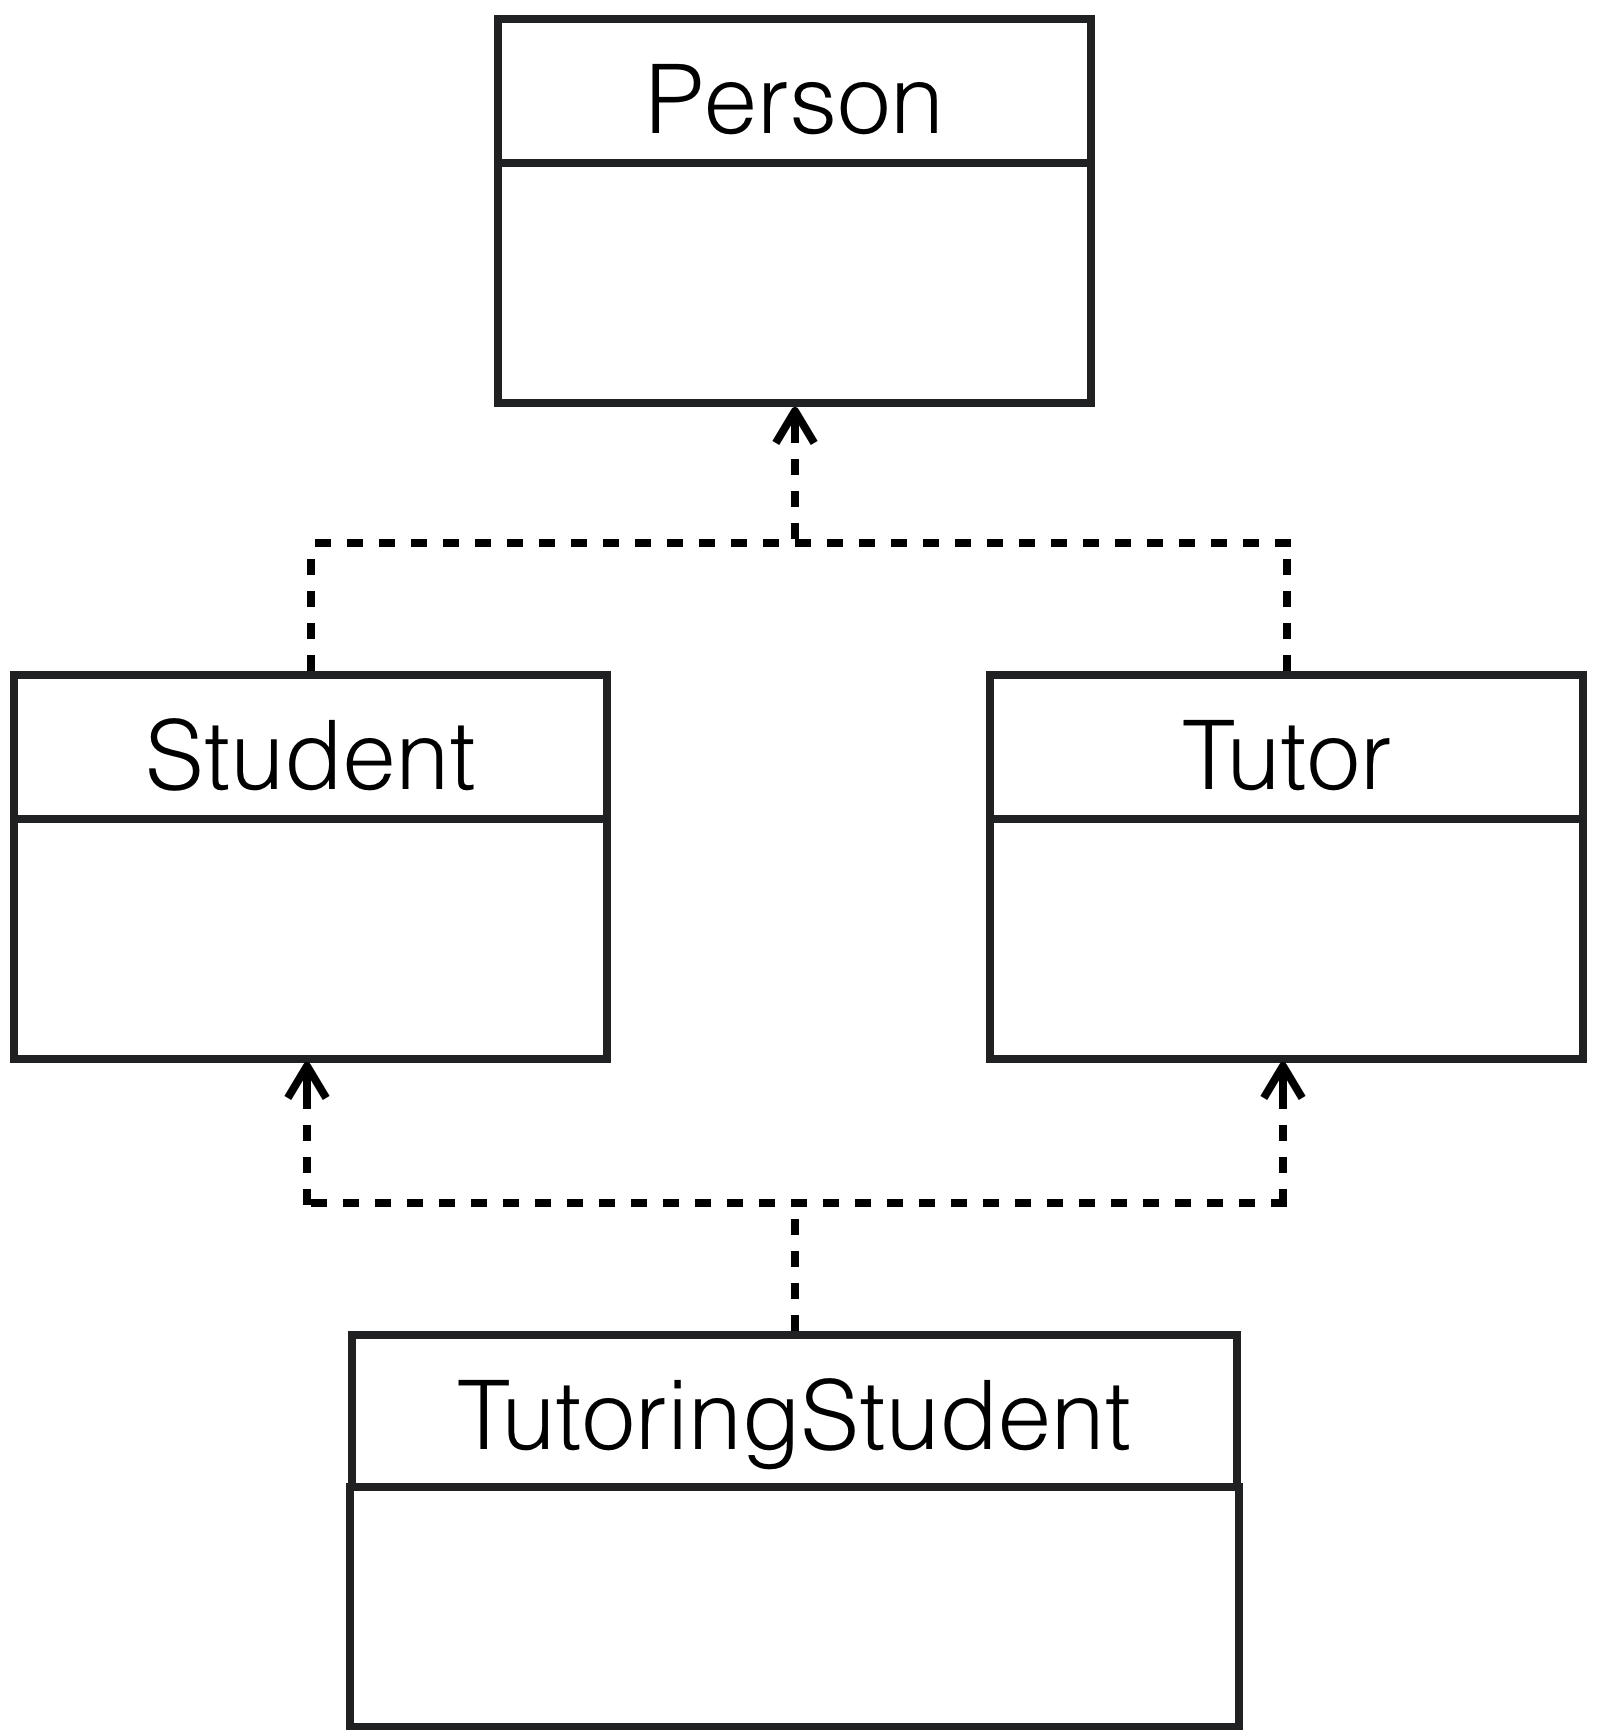
\includegraphics[width=0.34\textwidth]{images/multipleinheritance.png}
  \end{center}
  \caption{A UML class diagram with multiple inheritance}
  \label{fig:multipleinheritance}
\end{wrapfigure}

\subsubsection{Multiple Inheritance}
\label{sec:mulinh}
was first introduced by the predecessor of New Flavors, \emph{Flavors}. It allows classes to have multiple superclasses, thereby inheriting methods and attributes of each (see Figure \ref{fig:multipleinheritance}). The AthleticTeacher class defined by \mintinline{lisp}{(defclass athletic-teacher (teacher athlete) () )} would, if some inheritances from Teacher and Athlete are conflicting, prioritize the Teacher behavior, because it is listed first.  


\subsubsection{Method Combination}
\label{sec:metcom}
is an important addition to multiple inheritance, because it lets developers blend behavior together. The keywords \mintinline{lisp}{:before}, \mintinline{lisp}{:after}, and \mintinline{lisp}{:around} allow the specification of certain behavior to be added to a called method. \mintinline{lisp}{(defmethod method :after}\mintinline{lisp}{ ((teach teacher))}
    \mintinline{lisp}{()} would run additional behavior after the primary behavior defined for \mintinline{lisp}{method} for all Teacher. 


\subsubsection{Generic Functions}
\label{sec:genfun}
In Flavors, messages were sent to objects by calling the \mintinline{lisp}{send} function \mintinline{lisp}{(send object :message)}. New Flavors however introduced the \mintinline{lisp}{(message object)} notation, which required \mintinline{lisp}{message} to be \emph{generic}, meaning that it needed to be a globally defined interface (see Figure \ref{fig:genericfunction}). By calling the generic function, different behavior will ensue, depending on the type of the receiver provided as argument. If methods are defined that have no corresponding generic function, CLOS will add it automatically at compile time.


\begin{figure}[ht]
    \centering
    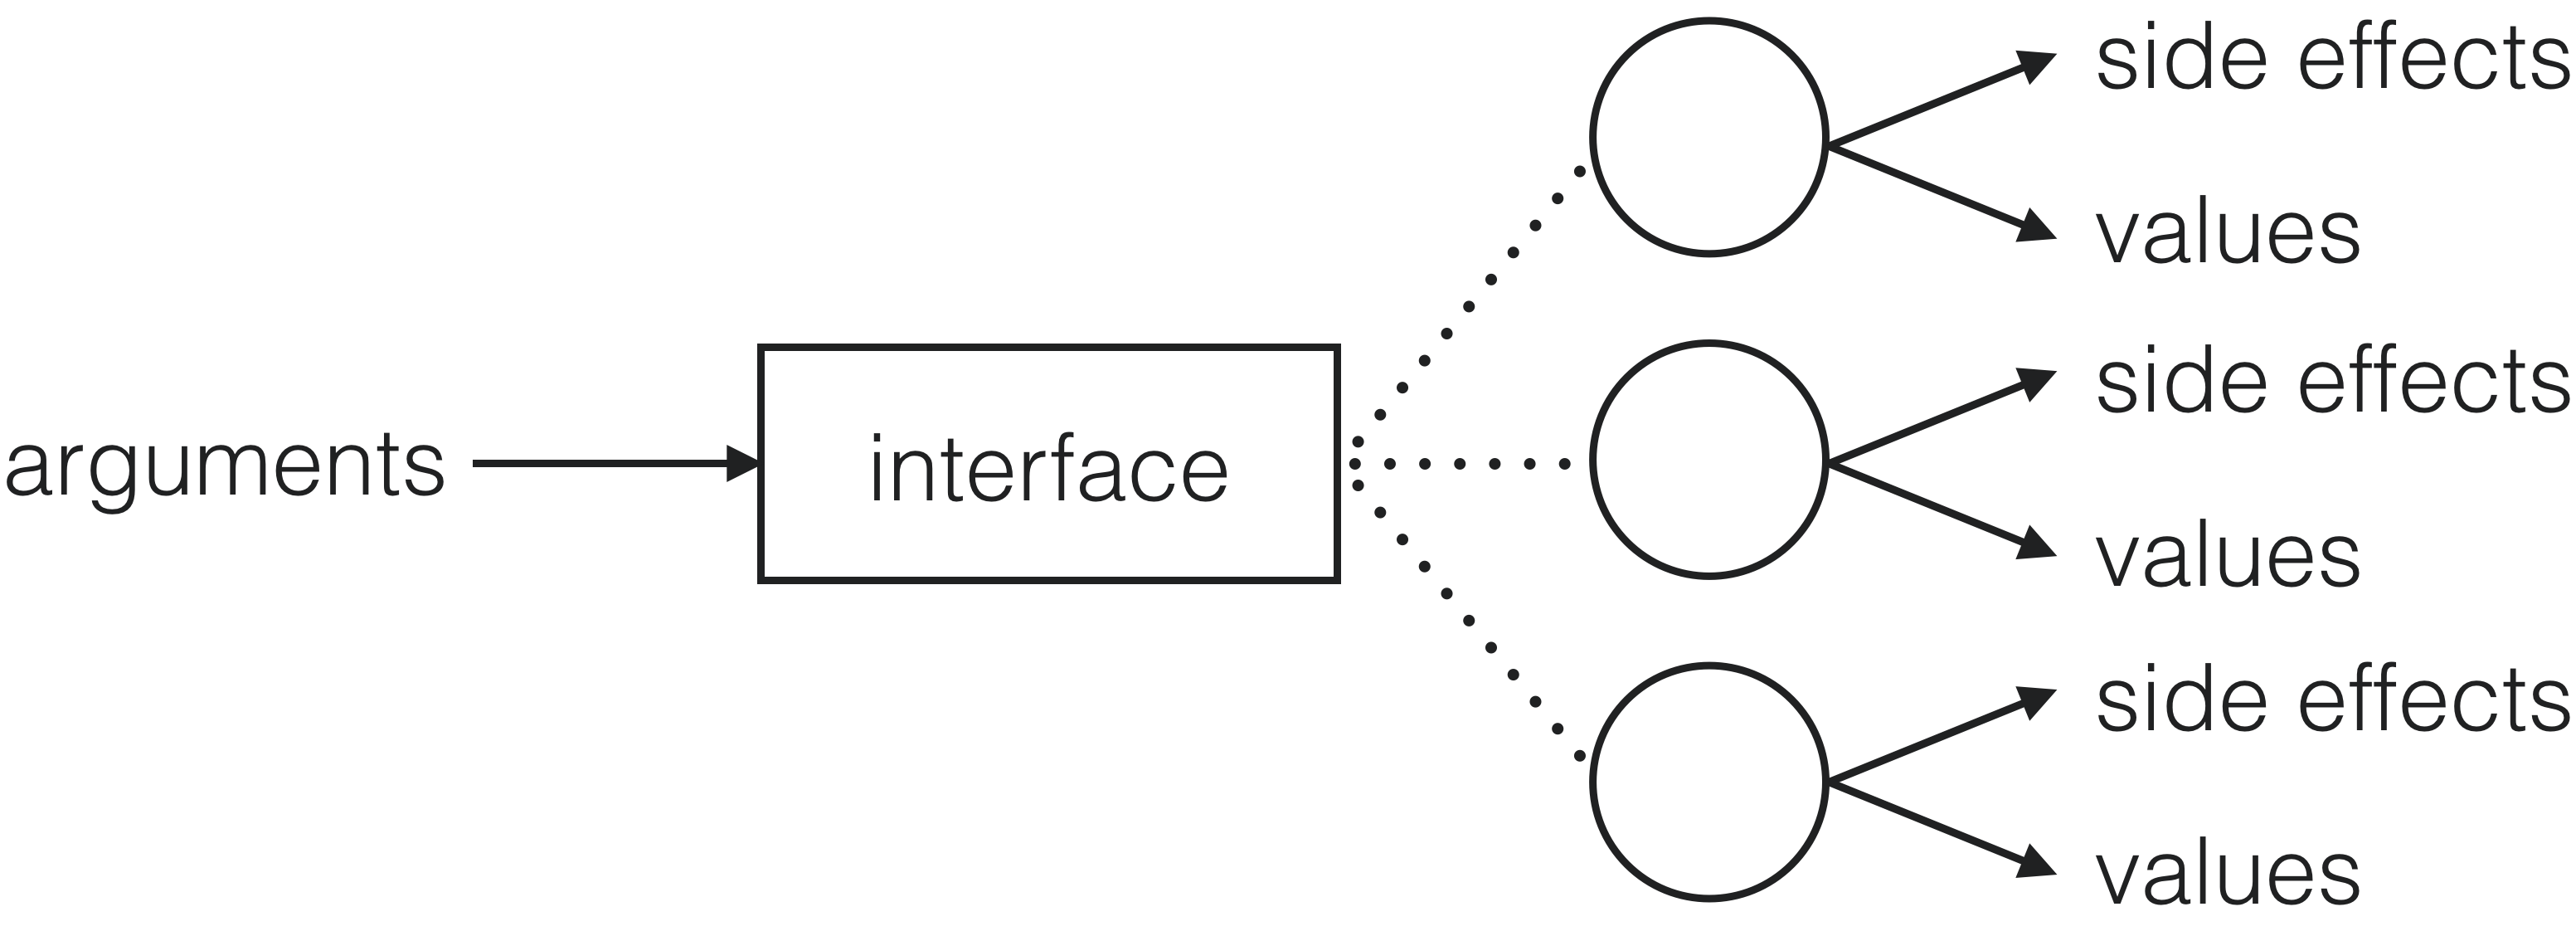
\includegraphics[width=0.5\textwidth]{images/genericfunction.png}
    \caption{The global interface provided by the generic function}
    \label{fig:genericfunction}
\end{figure}

\section{Approach}
\label{sec:approach}

It furthermore permits the storage in SQL database systems via object-relational mappers\footnote{A list of object-relational mappers for CLOS can be found at \url{http://www.cliki.net/ORM},  missing from the list is Mito (\url{https://github.com/fukamachi/mito}), both accessed: 2016-07-18} for easy access for non-Lisp programs.

\begin{itemize}
\item reasoning
\item problem step by step, show clos solution:
\item example case university: professors can also be "CEOs", students can also be tutors etc
\end{itemize}

\begin{itemize}
\item 3 concepts will be used
\item maybe give function that lets user add classes
\end{itemize}


\section{Implementation}
\label{sec:implementation}

\begin{listing}[]%ht]
\begin{minted}{lisp}

(defgeneric who-am-i (person)
      (:documentation "Makes the person describe themselves."))

(defmethod who-am-i ((p person))
    (format t "My name is ~d and I am ~d years old.~%" (person-name p) (person-age p)))

(defmethod who-am-i ((p teacher))
    (format t "My name is ~d and I am ~d years old.~%" (person-name p) (person-age p))
    (format t "I am a teacher and my subject is ~d.~%" (teacher-subject p)))

(defmethod who-am-i :after ((p teacher))
    (format t "I am a teacher and my subject is ~d.~%" (teacher-subject p)))

(defmethod who-am-i :after ((p athlete))
    (format t "I am an athlete and my sport is ~d.~%" (athlete-sport p)))

(defmethod who-am-i :around ((p athletic-teacher))
    (format t "Oh, hi!~%" )
    (let ((result (call-next-method)))
      (format t "Gotta sprint back to class, bye-bye!~%")
      result))

\end{minted}
\caption{The central macros provided by CLOS}
\label{lst:clossyntax}
\end{listing}



\begin{itemize}
\item give code details for concepts from Approach
\end{itemize}

\section{Evaluation}
\label{sec:evaluation}

\begin{itemize}
\item DSL type declaration is easily maintainable
\item using langs like Java (?) might be problematic, give example
\end{itemize}


\section{Conclusion}
\label{sec:conclusion}
Write me pl0x

\newpage
\nocite{*}
\bibliographystyle{splncs}
\bibliography{hopl-paper}

\end{document}